\section{Egy szabadsági fokú, gyengén csillapított rezgőrendszer mozgástörvénye}

\subsection*{Állandók meghatározása paraméteresen}
A gyengén csillapított rendszer ($\zeta < 1$) általános mozgástörvénye a következő alakú:
\begin{equation}
    x(t) = e^{-\zeta\omega_n t} \left( C_1 \cos(\omega_d t) + C_2 \sin(\omega_d t) \right)
\end{equation}
A sebesség kiszámításához deriváljuk az egyenletet:
\begin{equation}
    \dot{x}(t) = -\zeta\omega_n e^{-\zeta\omega_n t} \left( C_1 \cos(\omega_d t) + C_2 \sin(\omega_d t) \right) + e^{-\zeta\omega_n t} \left( -C_1 \omega_d \sin(\omega_d t) + C_2 \omega_d \cos(\omega_d t) \right)
\end{equation}
Alkalmazzuk a peremfeltételeket: $x(0) = 0$ és $\dot{x}(0) = v_0$.
Behelyettesítve $t = 0$-t a kitérés függvényébe:
\begin{equation}
    x(0) = 1 \cdot \left( C_1 \cdot 1 + C_2 \cdot 0 \right) = C_1 = 0
\end{equation}
Mivel $C_1 = 0$, a mozgástörvény egyszerűsödik, és az általános sebességképlet $t=0$ időpillanatára $C_1 = 0$ mellett a következőképp alakul:
\begin{equation}
    \dot{x}(0) = -\zeta\omega_n (0) + 1 \cdot \left( C_2 \omega_d \cdot 1 \right) = C_2 \omega_d = v_0
\end{equation}
Ebből $C_2$ számolható:
\begin{equation}
    C_2 = \frac{v_0}{\omega_d}
\end{equation}
Tehát a két paraméter: $C_1 = 0$ és $C_2 = \frac{v_0}{\omega_d}$. A mozgástörvény ennek okán: $x(t) = \frac{v_0}{\omega_d} e^{-\zeta\omega_n t} \sin(\omega_d t)$.

\subsection*{Rezgések amplitúdóinak változása}
A kialakuló rezgések amplitúdói az idő előrehaladtával az $e^{-\zeta\omega_n t}$ domináns szorzó miatt \textbf{exponenciálisan csökkenő füzér} (burkológörbe) mentén változnak. Az amplitúdók közötti arány, ha egy-egy $\Delta t = T_d$ periódust vizsgálunk,  állandó hányadost ad ki, amelyből a logaritmikus dekrementum is származtatható.

\subsection*{A kapott mozgástörvény ábrázolása (kitérés-idő diagram)}
Jelleghelyes kitérés-idő diagram megadott kezdeti feltételekkel (nulláról, meredeken induló kezdősebességgel):
\begin{figure}[H]
    \centering
    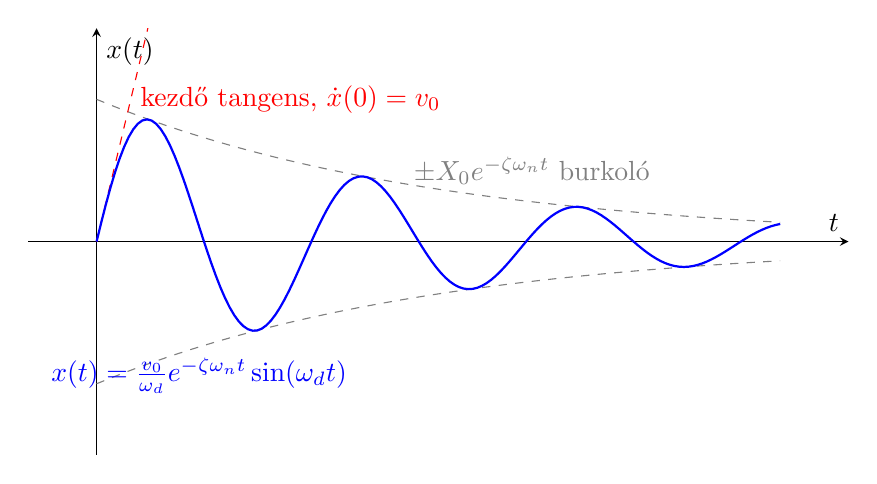
\begin{tikzpicture}
        \begin{axis}[
            width=12cm, height=7cm,
            axis lines=middle,
            xlabel={$t$},
            ylabel={$x(t)$},
            xmin=0, xmax=10,
            ymin=-1, ymax=1,
            xtick=\empty, ytick=\empty,
            enlargelimits=0.1,
            samples=150,
            domain=0:10
        ]
            % Envelope curves
            \addplot[dashed, gray, domain=0:10] {0.8*exp(-0.2*x)};
            \addplot[dashed, gray, domain=0:10] {-0.8*exp(-0.2*x)};
            
            % Initial velocity tangent
            \addplot[dashed, red, domain=0:2] {2*0.8*x};
            
            % Damped oscillation
            \addplot[thick, blue, domain=0:10] {0.8*exp(-0.2*x) * sin(deg(2*x))};

            \node[gray, right] at (axis cs: 4.5, 0.4) {$\pm X_0 e^{-\zeta\omega_n t}$ burkoló};
            \node[red, right] at (axis cs: 0.5, 0.8) {kezdő tangens, $\dot{x}(0) = v_0$};
            \node[blue, below] at (axis cs: 1.5, -0.6) {$x(t) = \frac{v_0}{\omega_d} e^{-\zeta\omega_n t} \sin(\omega_d t)$};
        \end{axis}
    \end{tikzpicture}
    \caption{Gyengén csillapított rendszer mozgástörvénye az előírt peremfeltételekkel.}
\end{figure}
